\subsection{Questions, workloads, and comparison hierarchy}
\label{sec:supplement}

The supplementary evaluation asks three questions: whether executable selection improves on optimized static paths, whether recent fusion artifacts can be compared on the same function, and whether subgraph results translate to complete inference.
Eager execution is a numerical and conventional execution reference, rather than a state-of-the-art optimization baseline.
The stronger comparisons use default compilation, max-autotune without internal CUDA Graphs, library SDPA, and FlashAttention-2.
We evaluate direct calls and controlled whole-chain CUDA Graph replay separately; results from these configurations are not pooled.

The GEMM matrix contains 21 shapes.
It retains the seven width-4096 pilot shapes, adds square widths 1024 and 8192 at $M\in\{1,128,512,2048\}$, and adds $(K,N)=(1024,3072)$ and $(3072,1024)$ at $M\in\{1,128,512\}$.
The nine attention cases retain the five pilot shapes and add causal prefill with $D=128$ at $S=512,2048$, and batch-eight GQA decode with $H_q=16$, $H_{kv}=8$, $D=64$, and $S_k=128,2048$.
For single-query decode all supplied KV entries are visible; applying an upper-left triangular mask would incorrectly exclude cached tokens.

We record PyTorch 2.5.1 with CUDA 12.1 and PyTorch 2.14.1 with CUDA 12.6 in separate environments.
Each admitted path must pass complete-output validation, including a second random seed and a larger-magnitude GEMM input.
The GEMM reference applies FP32 normalization to an FP16 product, with $10^{-3}$ relative and absolute tolerances; the attention FP32 reference uses $10^{-2}$ tolerances.
A rejected or unavailable candidate has no performance result and is excluded from the measured candidate minimum.
Paired comparisons with max-autotune use only their common admitted cases.

\subsection{Executed selection, timing, and calibration cost}
\label{sec:executed}

The supplementary executor invokes the selected callable on every measured call.
It never substitutes another row's median for its own latency.
Cache entries retain an exact tensor signature, including shape, strides, dtype, device, implementation identity, and device identity, alongside the analytical bucket.
An unprepared signature must be prepared before regular measurement or graph capture.
This prevents a bucket-level choice from silently reusing a different layout or precision.

The analytical rule and the $0.5R/2R$ thresholds are unchanged.
The main calibration scope remains ridge-plus-compute; analytical-only, ridge-only, and all-GEMM selection are separate ablations.
The ridge-only scope is an experimental variant rather than a change to the existing default.
Attention retains its fixed compiled-SDPA binding, so attention results do not demonstrate adaptive attention-plan selection.
Calibration uses three warmups and ten CUDA-event samples per candidate; the measurement helper also executes a separate ten-call host batch.
The reported calibration cost includes both batches and their synchronization.
Calibration samples are separate from regular samples.
Their elapsed setup cost is reported rather than incorporated into a steady-state speedup.

The operator protocol uses 50 warmups and 200 measured calls.
CUDA-event intervals and synchronized host batches are recorded separately.
Event intervals may include gaps caused by host dispatch and do not measure active-kernel time alone.
Host batch time includes actual callable dispatch and launches, with one final synchronization amortized over the batch.
Compiler preparation and numerical validation occur outside regular timing.
Manifests, individual samples, validation results, and available kernel/backend traces accompany each process.
Candidate timing order is logged: the first PyTorch 2.5.1 device series began with fixed order, and later series use seeded shuffling.
The two A40 devices are measured in separate processes, with three repetitions per device.
The PyTorch 2.14.1 GPU-1 series batches shapes within each repetition to avoid repeated framework startup; GPU-0 uses shape-isolated processes.
Analysis pairs both the shape and process, and bootstrap clusters retain each device/repetition; unavailable candidates and interrupted processes remain visible in the archive.

\subsection{Recent fusion artifacts and reproduction boundaries}
\label{sec:research-artifacts}

RedFuser and Neptune provide public 2026 fusion artifacts~\cite{Tang2026RedFuser,Zhao2026Neptune}.
Their attention bodies are compared as complete attention-plus-RMSNorm functions with the same compiled FP32 normalization epilogue.
This avoids appending an unoptimized normalization chain only to the research kernel.
The comparison concerns executable functions, not classifier accuracy or a reproduction of the authors' published speedups.
Official default schedules are identified explicitly; they are not presented as exhaustive autotuning results.

The RedFuser source is pinned to commit \texttt{56bf0b28}, and Neptune to \texttt{f7975011}.
The RedFuser generator requires compatibility handling for SymPy identity constants and unit-dimension TIR indices.
The exact patch is retained, and complete-output validation still rejects the regenerated kernel in the initial audit.
Its committed pre-generated kernel is evaluated separately, changing only literal tensor dimensions and launch extents.
Successful execution of that artifact does not establish successful automatic regeneration.
Unsupported causal, GQA, or head-dimension configurations are recorded rather than replaced by another implementation.
Neptune uses its official PyTorch 2.6/Triton 3.2 combination and an LLVM-enabled build.
Build failures, compatibility failures, numerical rejections, and measured paths are distinct outcomes.

The available hardware consists of Ampere A40 devices.
FA3/FA4 and ComFuse variants requiring Hopper/Blackwell facilities are therefore discussed as related work rather than claimed A40 reproductions.
Results from different compiler environments include matching in-environment baselines and are reported separately.

\subsection{Complete small-model inference}
\label{sec:small-system}

Large checkpoints are unnecessary for testing whether the selector survives integration into a complete execution graph.
We instantiate a six-layer Qwen3 architecture with hidden width 1024, intermediate width 3072, 16 query heads, eight KV heads, head dimension 64, an 8192-entry vocabulary, and tied embeddings.
The model contains 83,900,160 parameters, uses fixed random weights, and downloads no pretrained checkpoint.
The experiment measures architecture/runtime performance, not language-task accuracy.

The adapter replaces the actual projection--residual-add--RMSNorm region while retaining attention, RoPE, the MLP, residual flow, the KV cache, and the output head.
FP16 GEMM rounding is preserved through an explicit linear boundary; the compiled epilogue emulates the model's precision casts.
Without this boundary, compiler addmm rewriting changes the residual rounding position and fails the component numerical gate.
All admitted model variants pass full logits comparison on the same teacher-forced token history.

PyTorch workloads use batch sizes 1 and 8, prompt lengths 128 and 2048, and 64 decode steps.
All variants use the same outer default compilation configuration with internal CUDA Graphs disabled.
The original compiled model, a fixed-native adapter, a fixed-compiled adapter, and default SCIC are measured separately.
The fixed-native adapter exposes integration overhead; the fixed-compiled adapter tests whether adaptation is useful beyond a static choice.
The complete-model measurements include the real adapter and dispatcher costs.

Across the six device/process repetitions and four workloads, SCIC achieves host-time geometric-mean speed ratios of $0.870\times$ for prefill and $0.670\times$ for the 64-step decode loop relative to the original compiled model.
Both ratios indicate slowdowns.
The fixed-compiled adapter achieves $0.869\times$ and $0.675\times$, respectively.
These results show that pilot subgraph ratios cannot be interpreted as complete-model acceleration.
The opaque integration boundary and repeated runtime dispatch restrict the present implementation; calibration does not recover those costs.

\begin{figure*}[t]
  \centering
  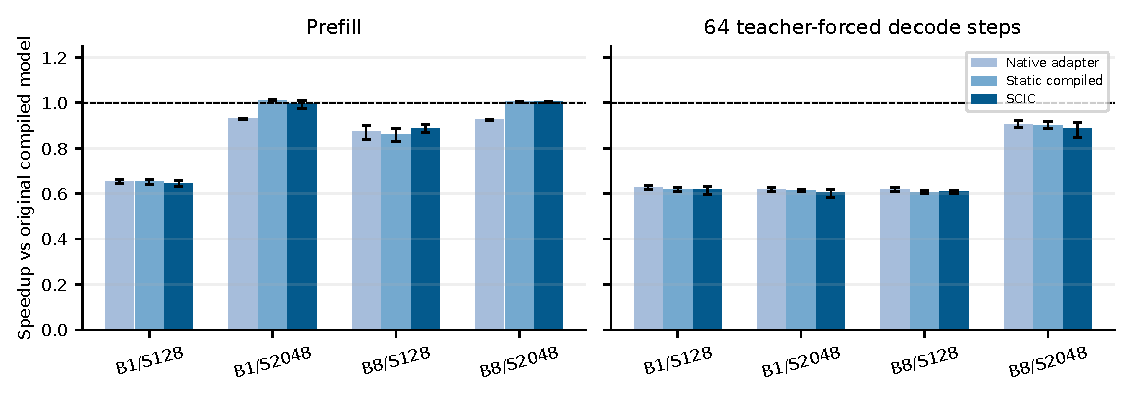
\includegraphics[width=\linewidth]{figures/fig_supplement_system.pdf}
  \caption{Complete random-weight small-Qwen3 inference. Speedup uses synchronized host batches relative to the original compiled model; values below one are slowdowns. Error bars are process-level bootstrap intervals. The workload includes the KV cache and output head, but uses teacher-forced tokens and does not measure task accuracy.}
  \label{fig:supplement-system}
\end{figure*}

\subsection{Measured optimized-baseline and research comparisons}

\label{sec:supplement-results}

Table~\ref{tab:supplement-selector} reports separately timed default SCIC against in-environment static paths. Ratios below one are slowdowns. Eager-relative gains do not imply an improvement over default compilation. The attention native reference is SDPA plus RMSNorm, not materialized attention. Max-autotune ratios use only common numerically admitted samples, whose counts are shown in parentheses.

\begin{table*}[t]

\centering\small

\caption{Executed ridge-plus-compute SCIC. Each ratio is a geometric mean of paired CUDA-event latencies. Direct calls and controlled whole-chain graph replay are separate. $n$ counts process/shape pairs; max-autotune uses common admitted pairs.}

\label{tab:supplement-selector}

\begin{tabular}{@{}lllrrrr@{}}

\toprule

PyTorch & Workload & Timing & $n$ & / native & / default & / max-no-graph ($n$) \\

\midrule

2.5.1 & GEMM & Direct & 126 & 1.225 & 0.890 & 0.839 (116) \\

2.5.1 & Attention & Direct & 54 & 1.045 & 0.830 & 0.831 (54) \\

2.5.1 & GEMM & Graph & 126 & 1.203 & 0.835 & 0.804 (116) \\

2.5.1 & Attention & Graph & 54 & 1.031 & 0.765 & 0.762 (54) \\

2.14.1 & GEMM & Direct & 126 & 1.161 & 0.922 & 0.834 (114) \\

2.14.1 & Attention & Direct & 54 & 0.982 & 0.880 & 0.900 (54) \\

2.14.1 & GEMM & Graph & 126 & 1.359 & 0.866 & 0.897 (114) \\

2.14.1 & Attention & Graph & 54 & 1.090 & 0.745 & 0.745 (54) \\

\bottomrule

\end{tabular}

\end{table*}

\begin{figure*}[t]

\centering

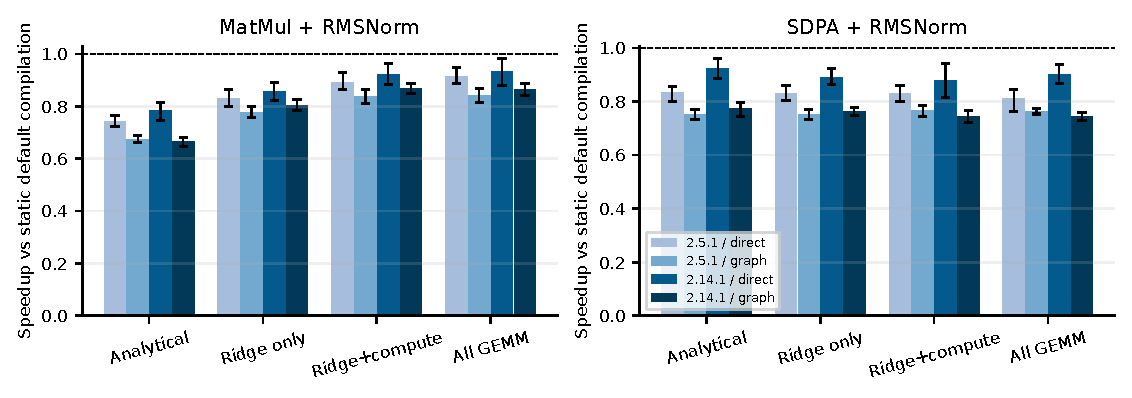
\includegraphics[width=\linewidth]{figures/fig_supplement_selector.pdf}

\caption{Independently timed selection relative to static default compilation, with process-bootstrap intervals. The analytical, ridge-only, default ridge-plus-compute, and all-GEMM scopes share the original $0.5R/2R$ rule. Attention always uses its fixed compiled-SDPA binding.}

\label{fig:supplement-selector}

\end{figure*}

For default-scope GEMM calibration, the following elapsed costs include probe calls and synchronization, after candidate preparation; they exclude compiler preparation and numerical auditing.

PyTorch 2.5.1 / none: 84 probes, median 9.264 ms, p95 146.433 ms.

PyTorch 2.5.1 / manual: 84 probes, median 7.360 ms, p95 145.861 ms.

PyTorch 2.14.1 / none: 84 probes, median 10.272 ms, p95 146.695 ms.

PyTorch 2.14.1 / manual: 84 probes, median 6.953 ms, p95 145.534 ms.

Table~\ref{tab:supplement-research} compares the admitted research artifacts against their matching compiler baselines. These are three process repetitions on one A40 per artifact, not a cross-environment ranking. RedFuser denotes the separately parameterized committed kernel, not successful regeneration.

\begin{table*}[t]

\centering\small

\caption{Complete attention-plus-compiled-RMSNorm research adapters. Default official schedules are used. Unsupported shapes have no timing. Max-no-graph uses the paired count in parentheses.}

\label{tab:supplement-research}

\begin{tabular}{@{}llrrrr@{}}

\toprule

Artifact & Timing & Shapes & Pairs & / default & / max-no-graph ($n$) \\

\midrule

RedFuser committed & Direct & 5 & 15 & 1.237 & 1.340 (15) \\

RedFuser committed & Graph & 5 & 15 & 1.028 & 0.936 (15) \\

Neptune TVM & Direct & 7 & 21 & 0.700 & 0.727 (21) \\

Neptune TVM & Graph & -- & 0 & unsupported & unsupported \\

Neptune Torch & Direct & 5 & 15 & 0.495 & 0.501 (15) \\

Neptune Torch & Graph & 5 & 15 & 0.958 & 0.983 (15) \\

\bottomrule

\end{tabular}

\end{table*}

The Neptune TVM/Triton bridge terminated with SIGSEGV during whole-chain CUDA Graph capture. Those process failures are retained; later captures are explicitly rejected rather than retried. This is an adapter compatibility boundary and does not invalidate its admitted direct calls.

Per-shape timings, process-bootstrap intervals, candidate admission status, available backend traces, and calibration costs remain in the supplementary analysis archive. The measured candidate minimum is limited to admitted executable paths and is not a global schedule optimum.

The official extracted Torch-callable Triton route requires Python integers for its launch configuration; the retained patch converts the TVM integer values without changing their values or schedules. The initial failed series is preserved separately. The admitted Torch-bridge cases exclude multi-kernel decode composition and GQA.

\paragraph{Framework-managed graphs}

The compiler-managed group retains its own direct default baseline. It measures reduce-overhead and max-autotune with the framework's internal graphs and ordinary, unmarked tensor arguments. Profiler traces contain input-copy kernels. Controlled manual replay instead captures fixed storage, and model parameters have their own framework treatment; these protocols are reported separately.

\begin{table}[t]

\centering\small

\caption{PyTorch 2.14.1 framework-managed graph modes relative to default compilation in the same process. Only admitted pairs enter each ratio.}

\label{tab:compiler-graphs}

\begin{tabular}{@{}llrr@{}}

\toprule

Workload & Mode & Pairs & / default \\

\midrule

attention & max-autotune & 27 & 0.871 \\

attention & reduce-overhead & 27 & 0.906 \\

gemm & max-autotune & 57 & 0.655 \\

gemm & reduce-overhead & 63 & 0.659 \\

\bottomrule

\end{tabular}

\end{table}

\paragraph{FlashAttention-2}

FlashAttention-2 with the same compiled FP32 normalization epilogue is available in the PyTorch 2.5.1 GPU-1 environment. Its admitted coverage is reported explicitly; the CUDA extension is ABI-specific and is not reused in the independent PyTorch 2.14.1 environment.

\begin{table}[t]

\centering\small

\caption{FlashAttention-2 plus compiled RMSNorm relative to the compiled SDPA chain in the same process.}

\label{tab:fa2-supplement}

\begin{tabular}{@{}lrrr@{}}

\toprule

Timing & Shapes & Pairs & / default \\

\midrule

Graph & 9 & 27 & 1.016 \\

Direct & 9 & 18 & 0.651 \\

\bottomrule

\end{tabular}

\end{table}


\subsection{Actual vLLM serving-engine integration}

\label{sec:vllm-system}

We additionally run the adapter inside vLLM 0.31.0's V1 AsyncLLM engine~\cite{Kwon2023vLLM}. The environment uses the CUDA-12.9 vLLM wheel and PyTorch 2.13.0+cu126 on the existing driver. Matching official torchvision/torchaudio CUDA-12.6 wheels and CPU torchcodec remove incidental CUDA-13 multimedia imports; package checks and the actual engine startup both pass.

The serving study uses 1 A40 device and 3 independent process repetitions per policy. GPU 0's sustained occupancy prevented its serving sequence from starting under the idle gate; the two-device operator and PyTorch-model studies remain separate.

The same complete small Qwen3 architecture uses seeded dummy weights, FP16, TP=1, and token-ID inputs. Each policy has its own worker process. All policies retain prefix caching, chunked prefill, the framework's default compilation/graphs, a 4096-token context limit, 16 maximum sequences, and 4096 batched tokens. Prompt lengths are 128 and 2048, concurrency is 1, 8, or 16, and each measured request generates 64 tokens. Two warmup batches precede 128 measured requests per workload. Unique deterministic prefixes prevent cross-request prefix reuse.

The comparison includes the original engine, fixed-native and fixed-compiled adapters, and SCIC. Every candidate passes component checks, and every admitted request's complete generated-token hash matches the original engine at the same seed, workload, and request ID. This verifies generated tokens rather than independently exported full-vocabulary logits. The PyTorch model experiment separately checks full logits.

Across six workloads and 3 paired process repetitions, SCIC's geometric-mean output-throughput ratio is $0.971\times$ relative to the original engine, with a process-bootstrap 95\% interval of $[0.961,0.978]$. This is an aggregate regression under the tested serving configuration; individual workloads differ. The fixed-compiled adapter's corresponding ratio is $0.992\times$. Table~\ref{tab:vllm-serving} reports absolute rates and tail TTFT alongside paired ratios.

\begin{table*}[t]

\centering\small

\caption{Actual vLLM V1 generation, 128 measured requests per process/workload, 64 output tokens per request. Rates are tokens/s and p95 TTFT is in milliseconds; displayed values are medians of per-process values. Ratios and intervals use paired processes. All candidate request token hashes match the original.}

\label{tab:vllm-serving}

\begin{tabular}{@{}rrrrrrr@{}}

\toprule

Input & Conc. & Orig. tok/s & SCIC tok/s & Ratio [95\% CI] & Orig. TTFT$_{95}$ & SCIC TTFT$_{95}$ \\

\midrule

128 & 1 & 538.9 & 531.4 & 0.980 [0.972, 0.986] & 12.45 & 13.78 \\

128 & 8 & 3573.6 & 3185.9 & 0.875 [0.843, 0.892] & 23.58 & 54.74 \\

128 & 16 & 5686.6 & 5382.3 & 1.001 [0.930, 1.053] & 38.62 & 60.55 \\

2048 & 1 & 513.8 & 503.4 & 0.968 [0.912, 1.015] & 14.05 & 15.79 \\

2048 & 8 & 2046.5 & 2148.9 & 1.032 [1.016, 1.053] & 96.49 & 103.95 \\

2048 & 16 & 2953.3 & 2841.1 & 0.977 [0.961, 0.986] & 137.91 & 154.92 \\

\bottomrule

\end{tabular}

\end{table*}

The client benchmark includes IPC, scheduling, KV-cache management, sampling, and streaming. Aggregate throughput also includes deterministic prompt construction; per-request TTFT starts after construction. Tokenizer and HTTP transport are excluded. ITL uses client-observed arrivals, so coalesced tokens share timestamps. Preparation outside regular measurement and any new-signature work inside measured requests retain their actual placement. The available final SCIC worker report records 84 prepared layer/signature entries and 469.467 ms of calibration; early statistics RPC failures are retained and are not replaced by inferred values.

\begin{figure*}[t]

\centering

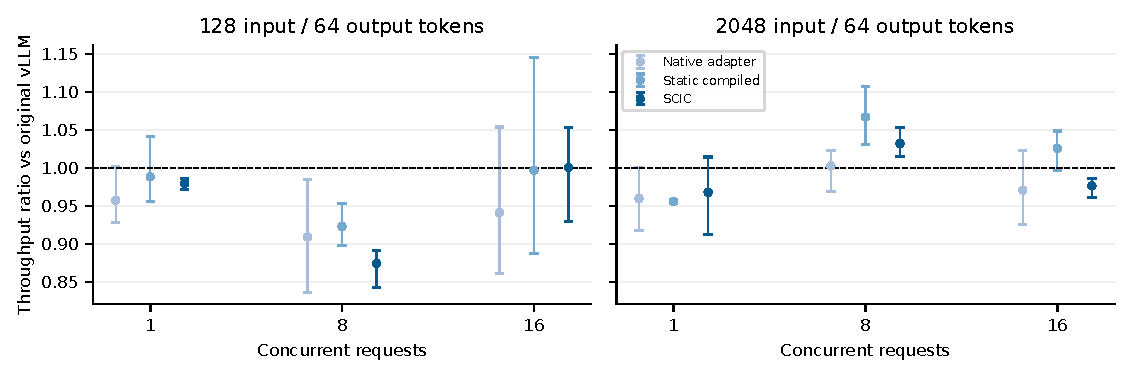
\includegraphics[width=\linewidth]{figures/fig_vllm_serving.pdf}

\caption{Token-validated vLLM serving throughput relative to the original optimized engine. Error bars resample independent process repetitions. The random-weight architecture and fixed batch arrivals do not establish pretrained task quality or production workload behavior.}

\label{fig:vllm-serving}

\end{figure*}


\subsection{Follow-up diagnosis of adapter overhead}

\label{sec:adapter-ablation}

The model slowdowns motivate a controlled diagnostic rather than a claim that threshold tuning will restore an advantage. We repeat all four HF workloads on two A40s, with three independent processes per device/workload, using PyTorch 2.5.1 and Transformers 4.51.3. The two device streams run concurrently on the same host; comparisons pair policies within a process and workload. The 95\% intervals resample six device/repetition clusters over the fixed workload matrix.

Initial trials interleaved profiler sessions and subsequent policy timings within a process. A separate intervention measures the same warmed original-model decode callable in three batches before and three after a CUDA-profiler session. After/before host-time speed ratios are $0.853\times$ on GPU 0 and $0.834\times$ on GPU 1, even after the profiler context exits. These within-process batches are descriptive checks, not independent repetitions. The initial trials are retained but excluded from every final latency and candidate summary; seed 0 is remeasured in processes that never initialize the profiler. The apparent inline advantage in those initial trials is therefore not used as acceleration evidence.

All seven arms use static outer compilation with internal CUDA Graphs disabled and precision-cast emulation enabled. Decode position tensors are allocated before timing. This common configuration differs from the earlier model protocol; its ratios are not pooled with those measurements. Every arm passes eager and compiled full-logit validation for the prefill and all 64 teacher-forced decode outputs at the unchanged $10^{-2}$ tolerances. Preparation, calibration, and profiler samples are excluded from the five-warmup/20-sample prefill and two-warmup/20-sample decode measurements; event samples and a separate synchronized host batch are retained.

The archived adapter constructs an exact signature twice per call. One-lookup dispatch reuses the cached entry directly. Prebinding freezes a separately validated callable for each layer's fixed prefill/decode phase; the caller checks the phase shape and the outer compiler supplies static guards. The prebound SCIC arm reuses the corresponding legacy pre-compilation SCIC decisions, avoiding a second selection experiment. These endpoints are fixed-workload specializations, not a general dynamic-shape runtime. The static inline arm removes the outer projection--add--norm custom operation and nested compiled callable, while retaining the opaque FP16 linear boundary and cast-before-affine semantics. It contains no adaptive selector or new MemMode/ComputeMode schedule. The one-lookup implementation is promoted to the general adapter while retaining the explicit two-lookup diagnostic control.

\begin{table*}[t]

\centering\small

\caption{Follow-up adapter ablation. Each entry is a geometric mean of 24 paired host-time speed ratios. Original denotes the original compiled model under this follow-up protocol. Fixed denotes the two-lookup fixed-compiled adapter. Values below one are slowdowns.}

\label{tab:adapter-ablation}

\begin{tabular}{@{}lrrrr@{}}

\toprule

Execution path & Prefill / original & Decode / original & Prefill / fixed & Decode / fixed \\

\midrule

Fixed compiled, two lookups & 0.867 & 0.649 & 1.000 & 1.000 \\

Fixed compiled, one lookup & 0.853 & 0.670 & 0.984 & 1.032 \\

Fixed compiled, prebound & 0.904 & 0.701 & 1.043 & 1.079 \\

Inline strict, static & 0.973 & 0.897 & 1.122 & 1.382 \\

SCIC, two lookups & 0.871 & 0.647 & 1.004 & 0.996 \\

SCIC, prebound & 0.889 & 0.703 & 1.026 & 1.083 \\

\bottomrule

\end{tabular}

\end{table*}

Relative to the two-lookup fixed adapter, one lookup achieves $0.984\times$ for prefill and $1.032\times$ for decode; prebinding achieves $1.043\times$ and $1.079\times$. The prebound fixed adapter remains at $0.904\times$ and $0.701\times$ relative to the original model. Prebound SCIC reaches $0.889\times$ and $0.703\times$. Removing signature lookup alone therefore does not recover the complete-model loss. The one-lookup prefill interval relative to fixed is [0.914, 1.024]; it includes one and retains an unusually slow host batch, so no stable prefill gain is claimed.

Static strict inlining reaches $0.973\times$ (95\% interval [0.969, 0.977]) for prefill and $0.897\times$ ([0.893, 0.901]) for decode relative to the original model. This result concerns integration of a static compiled path and does not establish an adaptive-selection advantage.

\begin{figure*}[t]

\centering

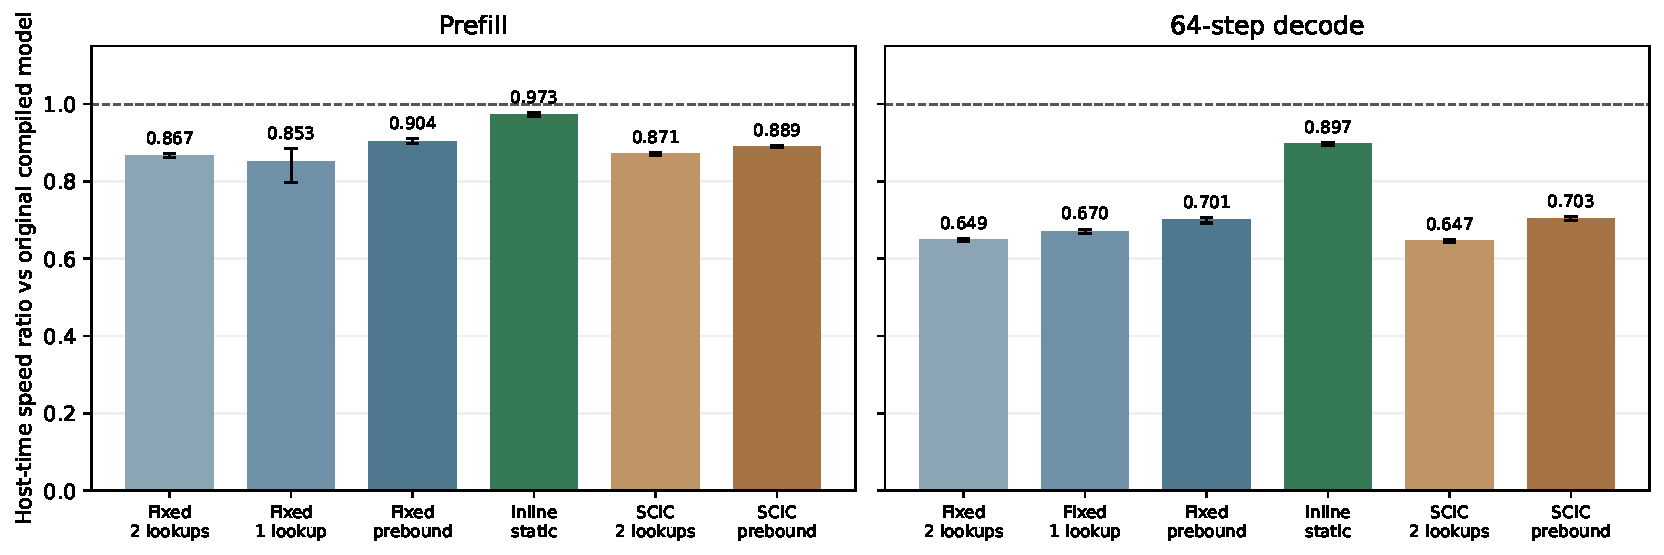
\includegraphics[width=\linewidth]{figures/fig_adapter_ablation.pdf}

\caption{Adapter diagnostics under a common follow-up protocol. Error bars resample device/repetition clusters; the original compiled model is the unit reference. Strict inlining is static, while the prebound paths specialize fixed prefill/decode signatures.}

\label{fig:adapter-ablation}

\end{figure*}

Profiler observations are retained in separate diagnostic processes; no process contributing to the final latency matrix starts a profiler. All 96 variant/workload/phase comparisons have the same CUDA-event count as their original-model reference. The opaque adapter paths enter seven compiled regions and perform seven Dynamo lookups per prefill, versus one for the original and inline paths; the 64-step decode counts are 448 versus 64. Prebinding eliminates exact-signature dispatch but retains these nested compiled calls. The archive retains CUDA-event names/counts and CPU operation counts. These are evidence about execution structure, not DRAM traffic or an isolated causal decomposition of kernel time.

A separate complete projection--residual--RMSNorm diagnostic measures six actual row counts: $M=1,8,128$ and $M=1024,2048,16384$, at width 1024 on the same six device/repetition clusters. It uses the initialized model's weight scale and unit normalization weights, preserving the $10^{-3}$ component gate. Of 36 paired shape/process measurements, native wins 25 host batches and 22 event medians. The optimistic per-shape minimum of native and compiled yields $1.155\times$ host and $1.130\times$ event speed ratios over fixed compilation. This minimum uses regular samples and is a diagnostic ceiling for this candidate set, not a measured selector or global schedule optimum. An initial arbitrary-normalization-weight smoke case failed the unchanged component gate; its rejection is retained and supplies no timing evidence for that signature.

A leave-one-seed-out check holds out both devices of each seed and selects each known shape's candidate using only event medians from the other two seeds. Its held-out ratios are $1.150\times$ for host batches and $1.127\times$ for events relative to fixed compilation; the best fixed candidate selected on training data is compiled in every fold. The held-out policy chooses native at $M=1,8,128,1024$ and compiled at $M=2048,16384$. This is offline evidence of ranking stability on known shapes, excluding dispatcher and calibration costs; it is not measured adaptive execution or unseen-shape generalization. The default analytical binding chooses compiled without probing memory-regime shapes, so it can miss the observed small-row native advantage. The crossover involves the strict adapter's existing execution paths and does not establish a transition between concrete resource-oriented kernel schedules.

The follow-up separates recoverable integration overhead from the unestablished value of analytical selection. The existing strict projection candidates have measurable local selection headroom, but adapter overhead prevents treating it as system acceleration. The next executable comparison should test all-shape empirical calibration against default SCIC and the best fixed adapter under the same invocation path. Demonstrating an intensity-guided scheduling advantage additionally requires concrete alternative schedules and evidence of the analytical feature's incremental value over empirical calibration. The diagnostic does not extend the optimized adapter to vLLM or validate pretrained normalization weights.

